% AIAA 3201 Project 2 report. CVPR 2027 author-kit style, camera-ready layout.
% Template source: https://github.com/cvpr-org/author-kit
% Build: latexmk -pdf -interaction=nonstopmode main.tex (from this directory).
\documentclass[times,10pt,twocolumn,letterpaper]{article}
\usepackage[final]{cvpr}
\usepackage{microtype}
\usepackage{multirow}
\usepackage{array}
\usepackage{placeins}
\definecolor{cvprblue}{rgb}{0.21,0.49,0.74}
\usepackage[pagebackref,breaklinks,colorlinks,allcolors=cvprblue]{hyperref}
\newcommand{\bestscore}[1]{\underline{\textbf{#1}}}
\def\confName{AIAA 3201 Project Report}
\def\confYear{2027}

\title{Few-Shot Industrial Anomaly Detection with Frozen DINOv2:\\
A Controlled Multi-Layer Feature Study}
\author{Ye Daojun\\Student ID: 50027656
\and Wang Yiming\\Student ID: 50027668}

\begin{document}
\maketitle

\begin{abstract}
Industrial inspection must recognize defects absent from training using only a few defect-free examples. We study six VisA product categories with an RGB template baseline, released AnomalyDINO, and one controlled improvement to its frozen DINOv2 descriptors. The improvement concatenates unit-normalized patch features from transformer blocks 8 and 11 before the original nearest-normal-neighbor search; references, calibration images, geometry, foreground masking, scoring, and evaluation remain fixed. Over 1/2/4/8 normal references and three reference groups, six-category image AUROC changes from 94.61/95.33/96.15/96.62\% to 94.74/95.47/96.45/96.85\%. Four-shot pixel AUROC barely changes (98.09\% to 98.12\%). In separate post-hoc experiments, pretrained score-map upsampling raises the two-layer method's pixel AP to 58.69\% over three reference groups, and fixed 448+672 image-scale fusion raises four-shot image AUROC to 96.74\%; the latter costs 3.46$\times$ query time and barely changes thresholded errors. These results expose the gap between ranking and calibrated decisions. GitHub: \url{https://github.com/yedaojun/AIAA3201-Project-2}.
\end{abstract}

\section{Introduction}
\label{sec:intro}
Industrial products can vary normally in pose, surface texture, background, and lighting. The same inspection system must also flag unseen scratches, contamination, and missing material. Exhaustively labeling defects is impractical, so the question is whether a few normal examples can define a useful boundary around normal appearance. A raw pixel comparison is easy to implement but assumes correspondence at nearly the same coordinates. A pretrained representation can compare local appearances even when objects move, yet its patch grid may dilute a tiny defect. This project investigates that trade-off under the exact six-category VisA protocol specified for AIAA 3201~\cite{zou2022visa}.

We implement three required stages. Part 1 selects the closest normal RGB template and uses a smoothed difference map. Part 2 reproduces released AnomalyDINO with a frozen DINOv2 ViT-S/14 backbone~\cite{damm2025anomalydino,oquab2024dinov2}. Part 3 tests a single primary hypothesis: combining an intermediate feature layer with the final layer should make local differences more visible while retaining the semantic stability of the official representation. The layer pair, equal normalization, and unchanged Part 2 foreground rule were fixed before inspecting the Part 3 test outcomes. Figure~\ref{fig:pipeline} summarizes the shared inputs and distinct scoring paths.

Our contributions are a paired six-category study of the RGB and official-feature baselines across four shot counts and three reference groups; a complete image- and pixel-level evaluation of the two-layer improvement with the exact same references; and an analysis that keeps favorable outcomes, regressions, and unresolved errors together. Additional directions are documented as secondary experiments. In particular, AnomalyCLIP has external anomaly supervision, and a review decision leaves some images unresolved. Neither should be silently equated with a like-for-like few-shot accuracy gain.

\begin{figure*}[t]
  \centering
  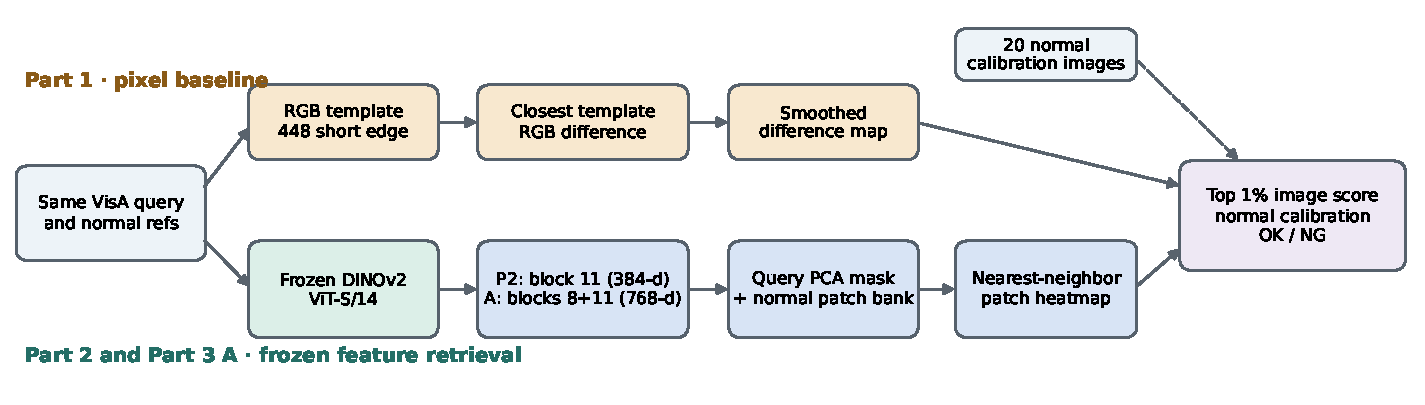
\includegraphics[width=\textwidth]{figures/pipeline.pdf}
  \caption{Our measured pipeline. Both required methods use the same normal reference filenames and test images. Part 1 compares RGB coordinates; Part 2 retrieves nearest normal DINOv2 patch features; the primary Part 3 change is the two-layer descriptor. The 20 additional normal images calibrate optional OK/NG demo thresholds but never enter a reference bank.}
  \label{fig:pipeline}
\end{figure*}

\section{Related Work}
\label{sec:related}
MVTec AD established a practical benchmark for normal-only industrial inspection~\cite{bergmann2019mvtec}; MVTec AD 2 later emphasized harder scenarios and evaluation conditions~\cite{hecklerkram2026mvtecad2}. VisA adds diverse product categories, official splits, and pixel masks used here~\cite{zou2022visa}. PaDiM estimates normal patch-feature distributions~\cite{defard2021padim}, while PatchCore concatenates intermediate and deep CNN features and stores representative normal patches for nearest-neighbor anomaly scoring~\cite{roth2022patchcore}. AnomalyDINO transfers this memory-based principle to frozen DINOv2 but uses its final ViT layer~\cite{damm2025anomalydino}. This contrast motivates testing whether an intermediate ViT layer adds local detail to the final-layer descriptor. EfficientAD explores the different objective of very low inference latency~\cite{batzner2024efficientad}.

Reconstruction and synthesis supply complementary signals. DRAEM learns from synthetic defects and reconstruction discrepancies~\cite{zavrtanik2021draem}; CutPaste uses pasted regions to create self-supervised anomalous examples~\cite{li2021cutpaste}. Our optional autoencoder and Direction C screening probe these ideas, but they are not treated as matched few-shot reproductions. DINOv2 learns transferable descriptors by large-scale self-supervision~\cite{oquab2024dinov2}. AnomalyDINO uses these frozen patch descriptors and a normal memory bank, which makes unseen-defect detection possible without fitting a target anomaly classifier~\cite{damm2025anomalydino}. AnomalyCLIP instead learns object-agnostic normal/abnormal prompt representations from an external anomaly dataset~\cite{zhou2024anomalyclip}. Its different supervision matters when interpreting fusion results. AnyUp supplies pretrained image-guided feature upsampling~\cite{wimmer2026anyup}; we test a score-map adaptation separately rather than presenting it as a native component of AnomalyDINO.

\section{Method}
\label{sec:method}
\subsection{Shared data and decision protocol}
We use VisA's official \texttt{1cls} split and the six required classes: candle, capsules, cashew, chewinggum, fryum, and pipe\_fryum. The test set contains 360 normal and 600 anomalous images. For every class, the first 20 normal training files in filename order are reserved for score calibration and excluded before reference selection. The remaining reference filenames are fixed for 1, 2, 4, and 8 shots and three official reference groups (seeds 0, 1, and 2). These are ordered reference selections, not three retrained backbones. All required methods use the same test images and annotations.

For the Part 1 demonstration, the category threshold is the 95th percentile of the 20 normal calibration image scores. We apply the same normal-only decision policy separately to the Part 2 and Part 3 demos. It determines \texttt{OK}/\texttt{NG}, not AUROC. Detection and localization AUROC always use raw, unthresholded scores; calibration images never fit a model or enter a memory bank.

\subsection{Part 1: closest-template difference}
Images are resized bicubically to a 448-pixel short edge, preserving aspect ratio, then cropped on the bottom and right to dimensions divisible by 14. For each test image, we choose the normal reference with the lowest whole-image mean absolute RGB difference. The per-pixel map is the rounded channel-mean absolute difference, smoothed by a Gaussian with $\sigma=2$ working pixels and restored to the original size. The image score is the mean of the highest 1\% of smoothed pixel values, divided by 255. We use neither ECC registration nor morphological cleanup. Thus normal displacement, background variation, or illumination can create large residuals even when no product defect exists.

\subsection{Part 2: official AnomalyDINO}
We run the released AnomalyDINO components with \texttt{dinov2\_vits14}, agnostic preprocessing, 448-pixel short edge, reference rotations, and CPU FAISS search~\cite{damm2025anomalydino}. The backbone remains frozen. Let $f_{11}(p)$ be the final-layer descriptor of query patch $p$ and $\mathcal B$ the unit-normalized descriptors from rotated normal references. The official score is the nearest-neighbor cosine distance, implemented by half squared Euclidean distance between unit vectors:
\begin{equation}
  d(p,\mathcal B)=\min_{b\in\mathcal B}\frac{\lVert\hat f_{11}(p)-\hat b\rVert_2^2}{2}.
  \label{eq:distance}
\end{equation}
The official PCA rule masks selected query background patches. Distances placed back on the query grid form a coarse map; its original-resolution reconstruction uses the official bilinear interpolation and Gaussian smoothing. If $d_{(1)}\geq\cdots\geq d_{(P)}$ are patch distances in descending order, the image score is
\begin{equation}
  S(I)=\frac{1}{k}\sum_{j=1}^{k}d_{(j)},\qquad k=\max(1,\lfloor0.01P\rfloor).
  \label{eq:score}
\end{equation}
The memory bank stores product-specific normality, while transferable frozen features allow a defect to differ from known normal patches without having been seen as a labeled target defect. Retrieval is not tied to an identical pixel position, but the query patch keeps its grid location for heatmap display. A 14-pixel sampling stride and the restored smooth map limit precise boundaries for sparse damage.

\subsection{Part 3: two-layer frozen descriptors}
Our primary improvement changes only the representation before the same nearest-neighbor search. We extract intermediate transformer block 8 and final block 11 (zero-based) at the same input resolution. Each layer's descriptor is normalized separately, then concatenated. FAISS normalization makes its effective vector
\begin{equation}
  f_A(p)=\frac{1}{\sqrt 2}\left[\frac{f_8(p)}{\lVert f_8(p)\rVert_2};
  \frac{f_{11}(p)}{\lVert f_{11}(p)\rVert_2}\right].
  \label{eq:two_layer}
\end{equation}
The final-layer query PCA mask, unmasked rotated-reference bank construction, distance definition, top-1\% image score, calibration rule, and original-resolution map restoration are otherwise unchanged. No VisA weights are trained. This isolates feature-layer choice better than changing backbone, reference sampling, preprocessing, and postprocessing simultaneously.

\section{Evaluation Protocol}
\label{sec:protocol}
For every class, shot count, and reference group, we evaluate all official test images. Image AUROC ranks normal against anomalous images using $S(I)$. Pixel AUROC uses the raw restored floating heatmap at every original-resolution pixel, including all normal images with zero masks. We first compute each category's AUROC, average six categories equally within a reference group, then report the mean and \emph{sample} standard deviation over groups 0, 1, and 2. We never rescale each test heatmap separately for AUROC. Exact pixel average precision (AP) is evaluated on original-resolution maps with all normal zero masks: Table~\ref{tab:pixelap} covers four shots and all three reference groups; the exploratory 448+672 branch additionally covers all four shot counts. Ground-truth masks appear only in evaluation and display crops.

The paired benchmark serially processes 120 fixed queries on one RTX 4060 Laptop GPU, ten normal and ten anomalous per category. All five model paths are warmed and stay resident in one process; query order alternates. Each synchronized timing includes image decode, feature extraction, retrieval, scoring, and original-size map restoration, but excludes model and reference setup, file output, and metric computation. Peak memory is PyTorch's allocated GPU tensor memory during a query, including resident weights, not total device occupancy. RGB and isolated stage diagnostics use different boundaries and are reported separately.

\paragraph{Scope and fairness guardrails.} A is the pre-fixed primary feature comparison. The 672 branch and its equal fusion were devised after seeing errors on this same test split; matched references and three groups measure sensitivity but do not provide an untouched validation set. AnyUp adds a pretrained upsampler after retrieval, while AnomalyCLIP uses external anomaly labels. A \texttt{REVIEW} decision is unresolved until a human acts, and test-derived FPR operating points are evaluation summaries, never deployment thresholds.

\section{Results}
\label{sec:results}
\subsection{Required methods across all shots}
Table~\ref{tab:allshots} reports all 72 category/shot/group configurations per required method. The RGB template image AUROC ranges from 52.67\% to 61.00\%, while frozen DINO reaches 94.61--96.62\%. The large gap is consistent with strict coordinate-wise RGB differences responding to harmless position and appearance changes. For example, a normal capsules image, \texttt{good/016.JPG}, is a template false positive at four shots/group 0 (score 0.5202 versus threshold 0.4937); DINO correctly accepts it (0.1175 versus 0.1531). Figure~\ref{fig:templatefp} uses four-decimal score labels so this value agrees with the text. The image shows alignment sensitivity without isolating pose from illumination experimentally. Figure~\ref{fig:shot} plots the measured trends.

\begin{table*}[t]
\centering
\caption{Six-category macro AUROC (\%, mean $\pm$ sample SD across three reference groups). Pixel AUROC includes normal test images with zero masks. $\Delta$ is A minus Official DINO in percentage points from displayed means; bold marks the better paired result. Reference filenames are shared.}
\label{tab:allshots}
\setlength{\tabcolsep}{3.1pt}
\scriptsize
\begin{tabular}{c cccc cccc}
\toprule
\multirow{2}{*}{Refs} & \multicolumn{4}{c}{Image AUROC} & \multicolumn{4}{c}{Pixel AUROC}\\
 & RGB template & Official DINO & Two-layer A & $\Delta$ & RGB template & Official DINO & Two-layer A & $\Delta$\\
\midrule
1 & $52.67\pm0.97$ & $94.61\pm1.03$ & $\mathbf{94.74\pm0.99}$ & +0.13 & $76.71\pm0.84$ & $\mathbf{97.76\pm0.07}$ & $97.71\pm0.06$ & $-0.05$\\
2 & $55.84\pm4.65$ & $95.33\pm0.57$ & $\mathbf{95.47\pm0.54}$ & +0.14 & $77.22\pm0.60$ & $97.92\pm0.08$ & $97.92\pm0.04$ & 0.00\\
4 & $57.80\pm4.31$ & $96.15\pm0.49$ & $\mathbf{96.45\pm0.38}$ & +0.30 & $77.12\pm0.38$ & $98.09\pm0.03$ & $\mathbf{98.12\pm0.05}$ & +0.03\\
8 & $61.00\pm0.36$ & $96.62\pm0.70$ & $\mathbf{96.85\pm0.74}$ & +0.23 & $77.46\pm0.39$ & $98.21\pm0.02$ & $\mathbf{98.25\pm0.05}$ & +0.04\\
\bottomrule
\end{tabular}
\end{table*}

\begin{figure*}[t]
  \centering
  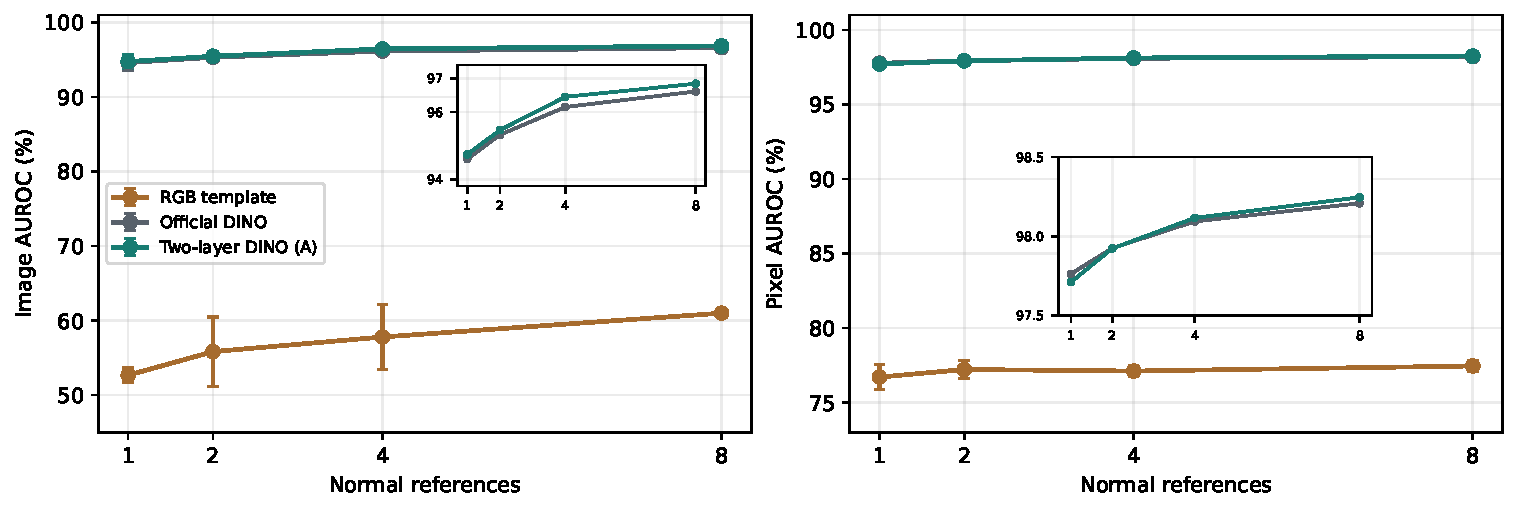
\includegraphics[width=.86\textwidth]{figures/shot_curves.pdf}
  \caption{The full-shot mean AUROCs from Table~\ref{tab:allshots}; error bars are sample SD across three reference groups. The two-layer gain is primarily in image ranking.}
  \label{fig:shot}
\end{figure*}

\begin{figure*}[t]
  \centering
  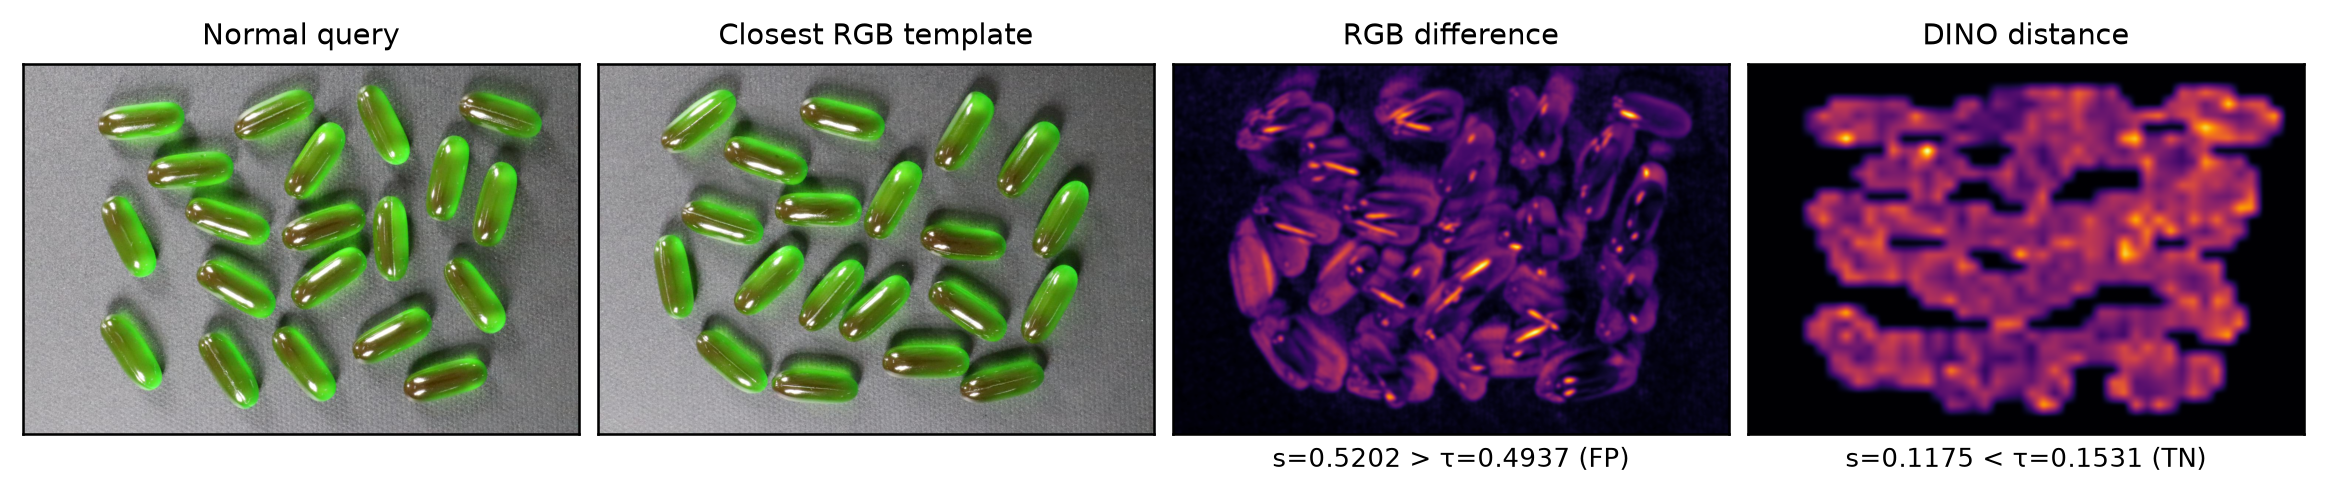
\includegraphics[width=.93\textwidth]{figures/template_false_positive.png}
  \caption{A normal capsules query at four shots/seed 0. The nearest RGB template differs in benign appearance, producing an RGB false alarm (FP); frozen DINO accepts the same query (TN). The two heatmaps have method-specific scales; the scores and normal-calibrated thresholds $\tau$ determine decisions.}
  \label{fig:templatefp}
\end{figure*}

\begin{figure*}[t]
  \centering
  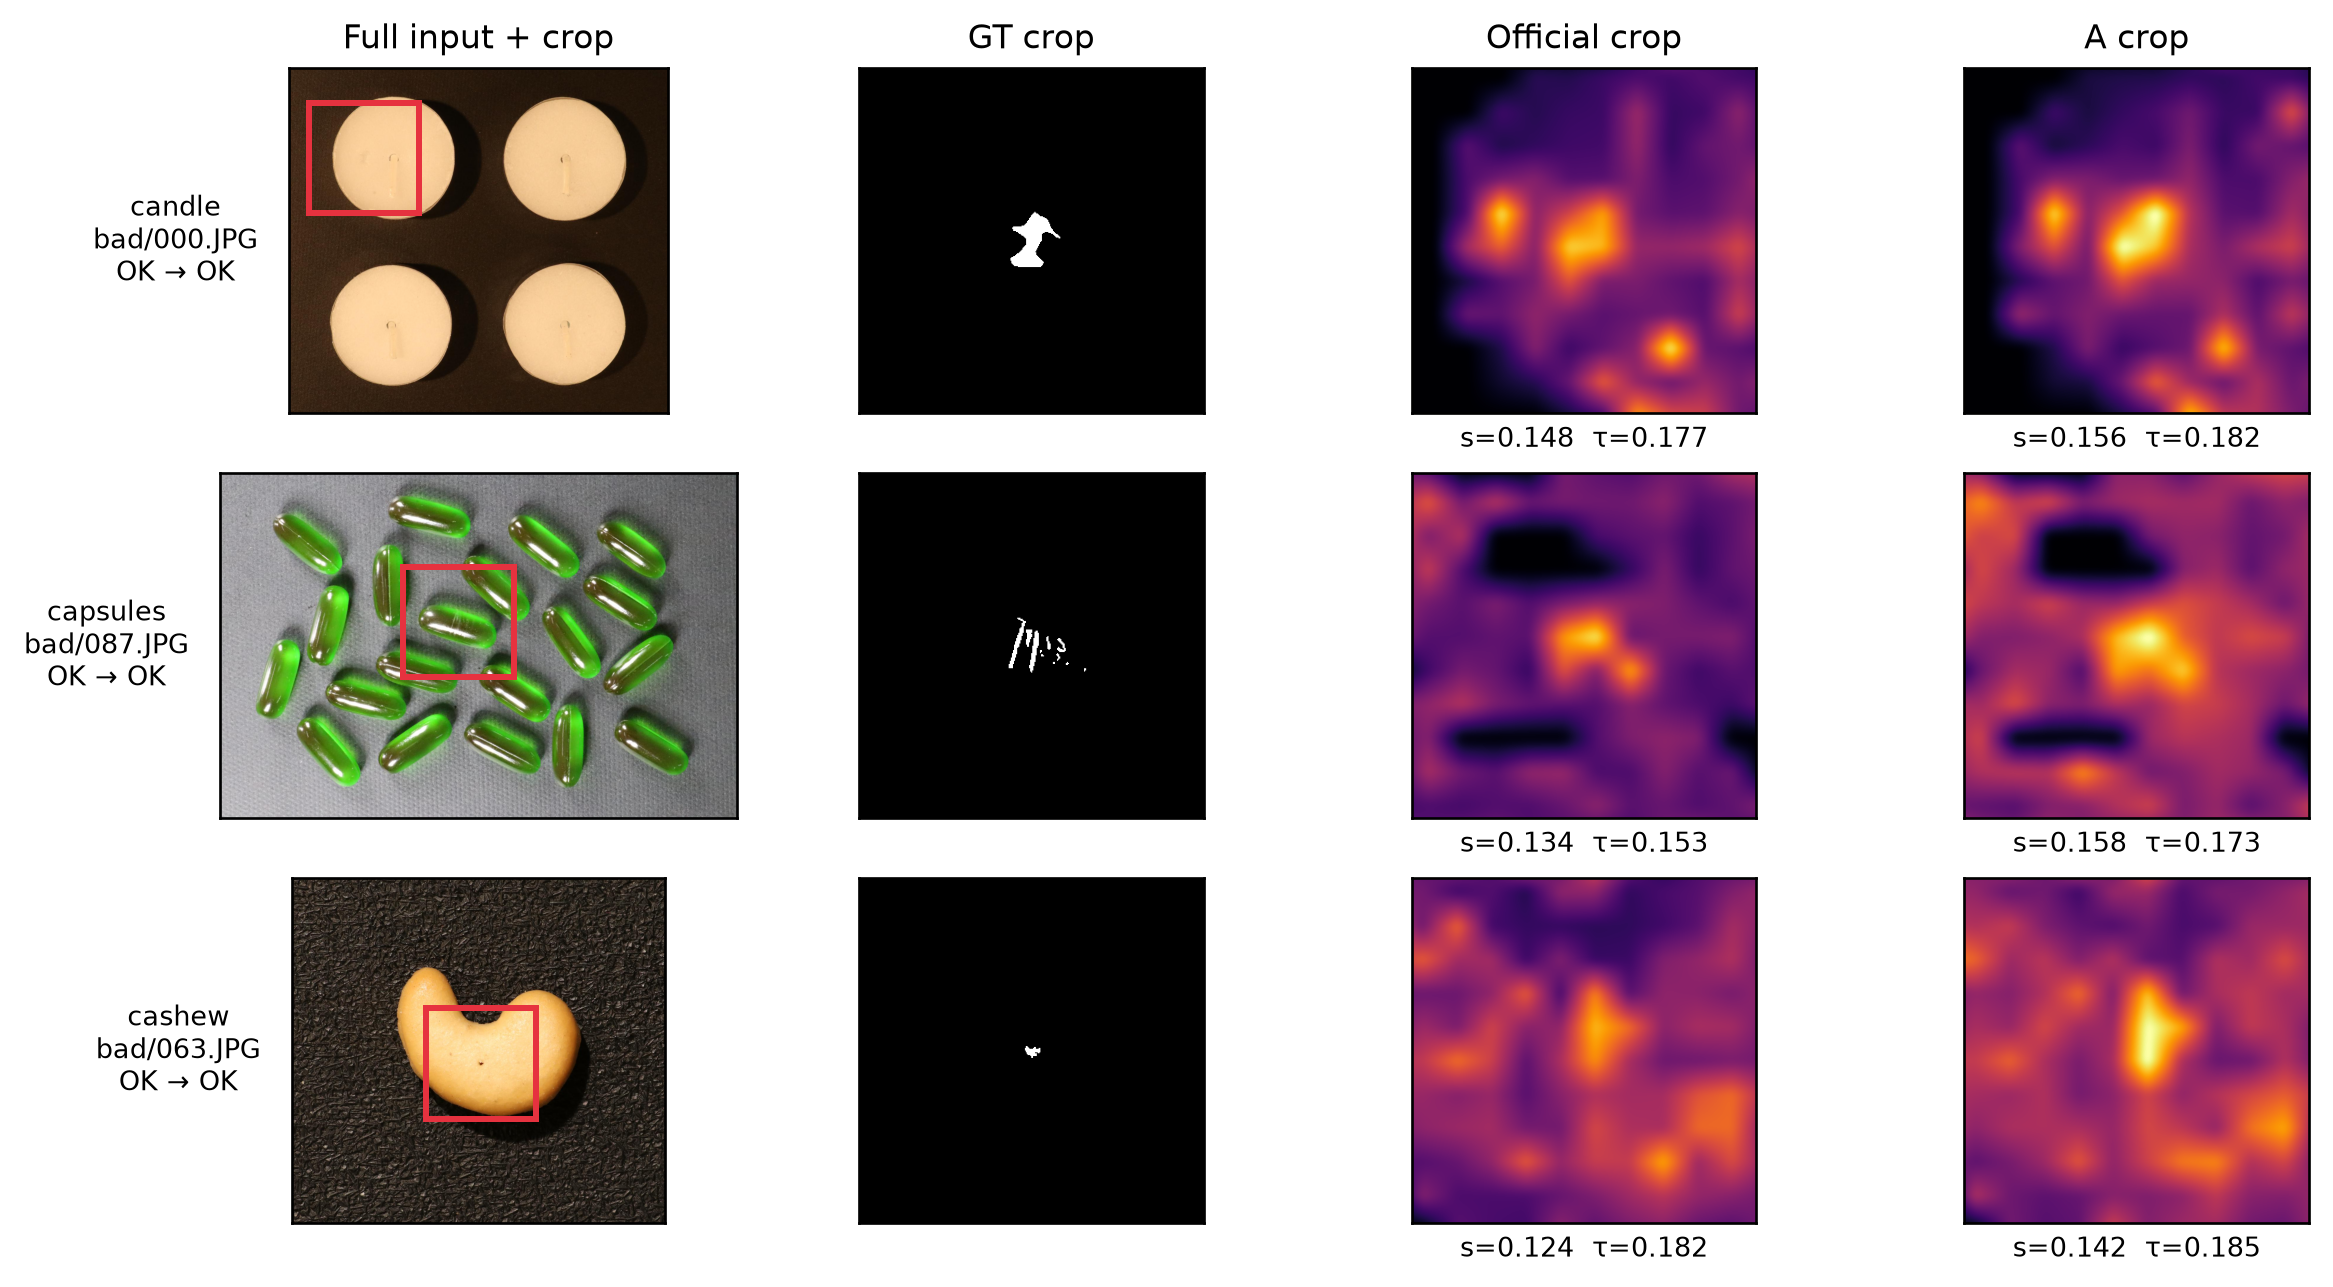
\includegraphics[width=.98\textwidth]{figures/difficult_cases_1.png}
  \caption{Three remaining false negatives. The full input shows the red display-crop box, followed by the binary ground-truth crop and matched-scale official/A heatmap crops. \texttt{OK} means each anomaly is still missed. Values below heatmaps are raw image scores $s$ and independently normal-calibrated thresholds $\tau$.}
  \label{fig:cases1}
\end{figure*}

\begin{figure*}[t]
  \centering
  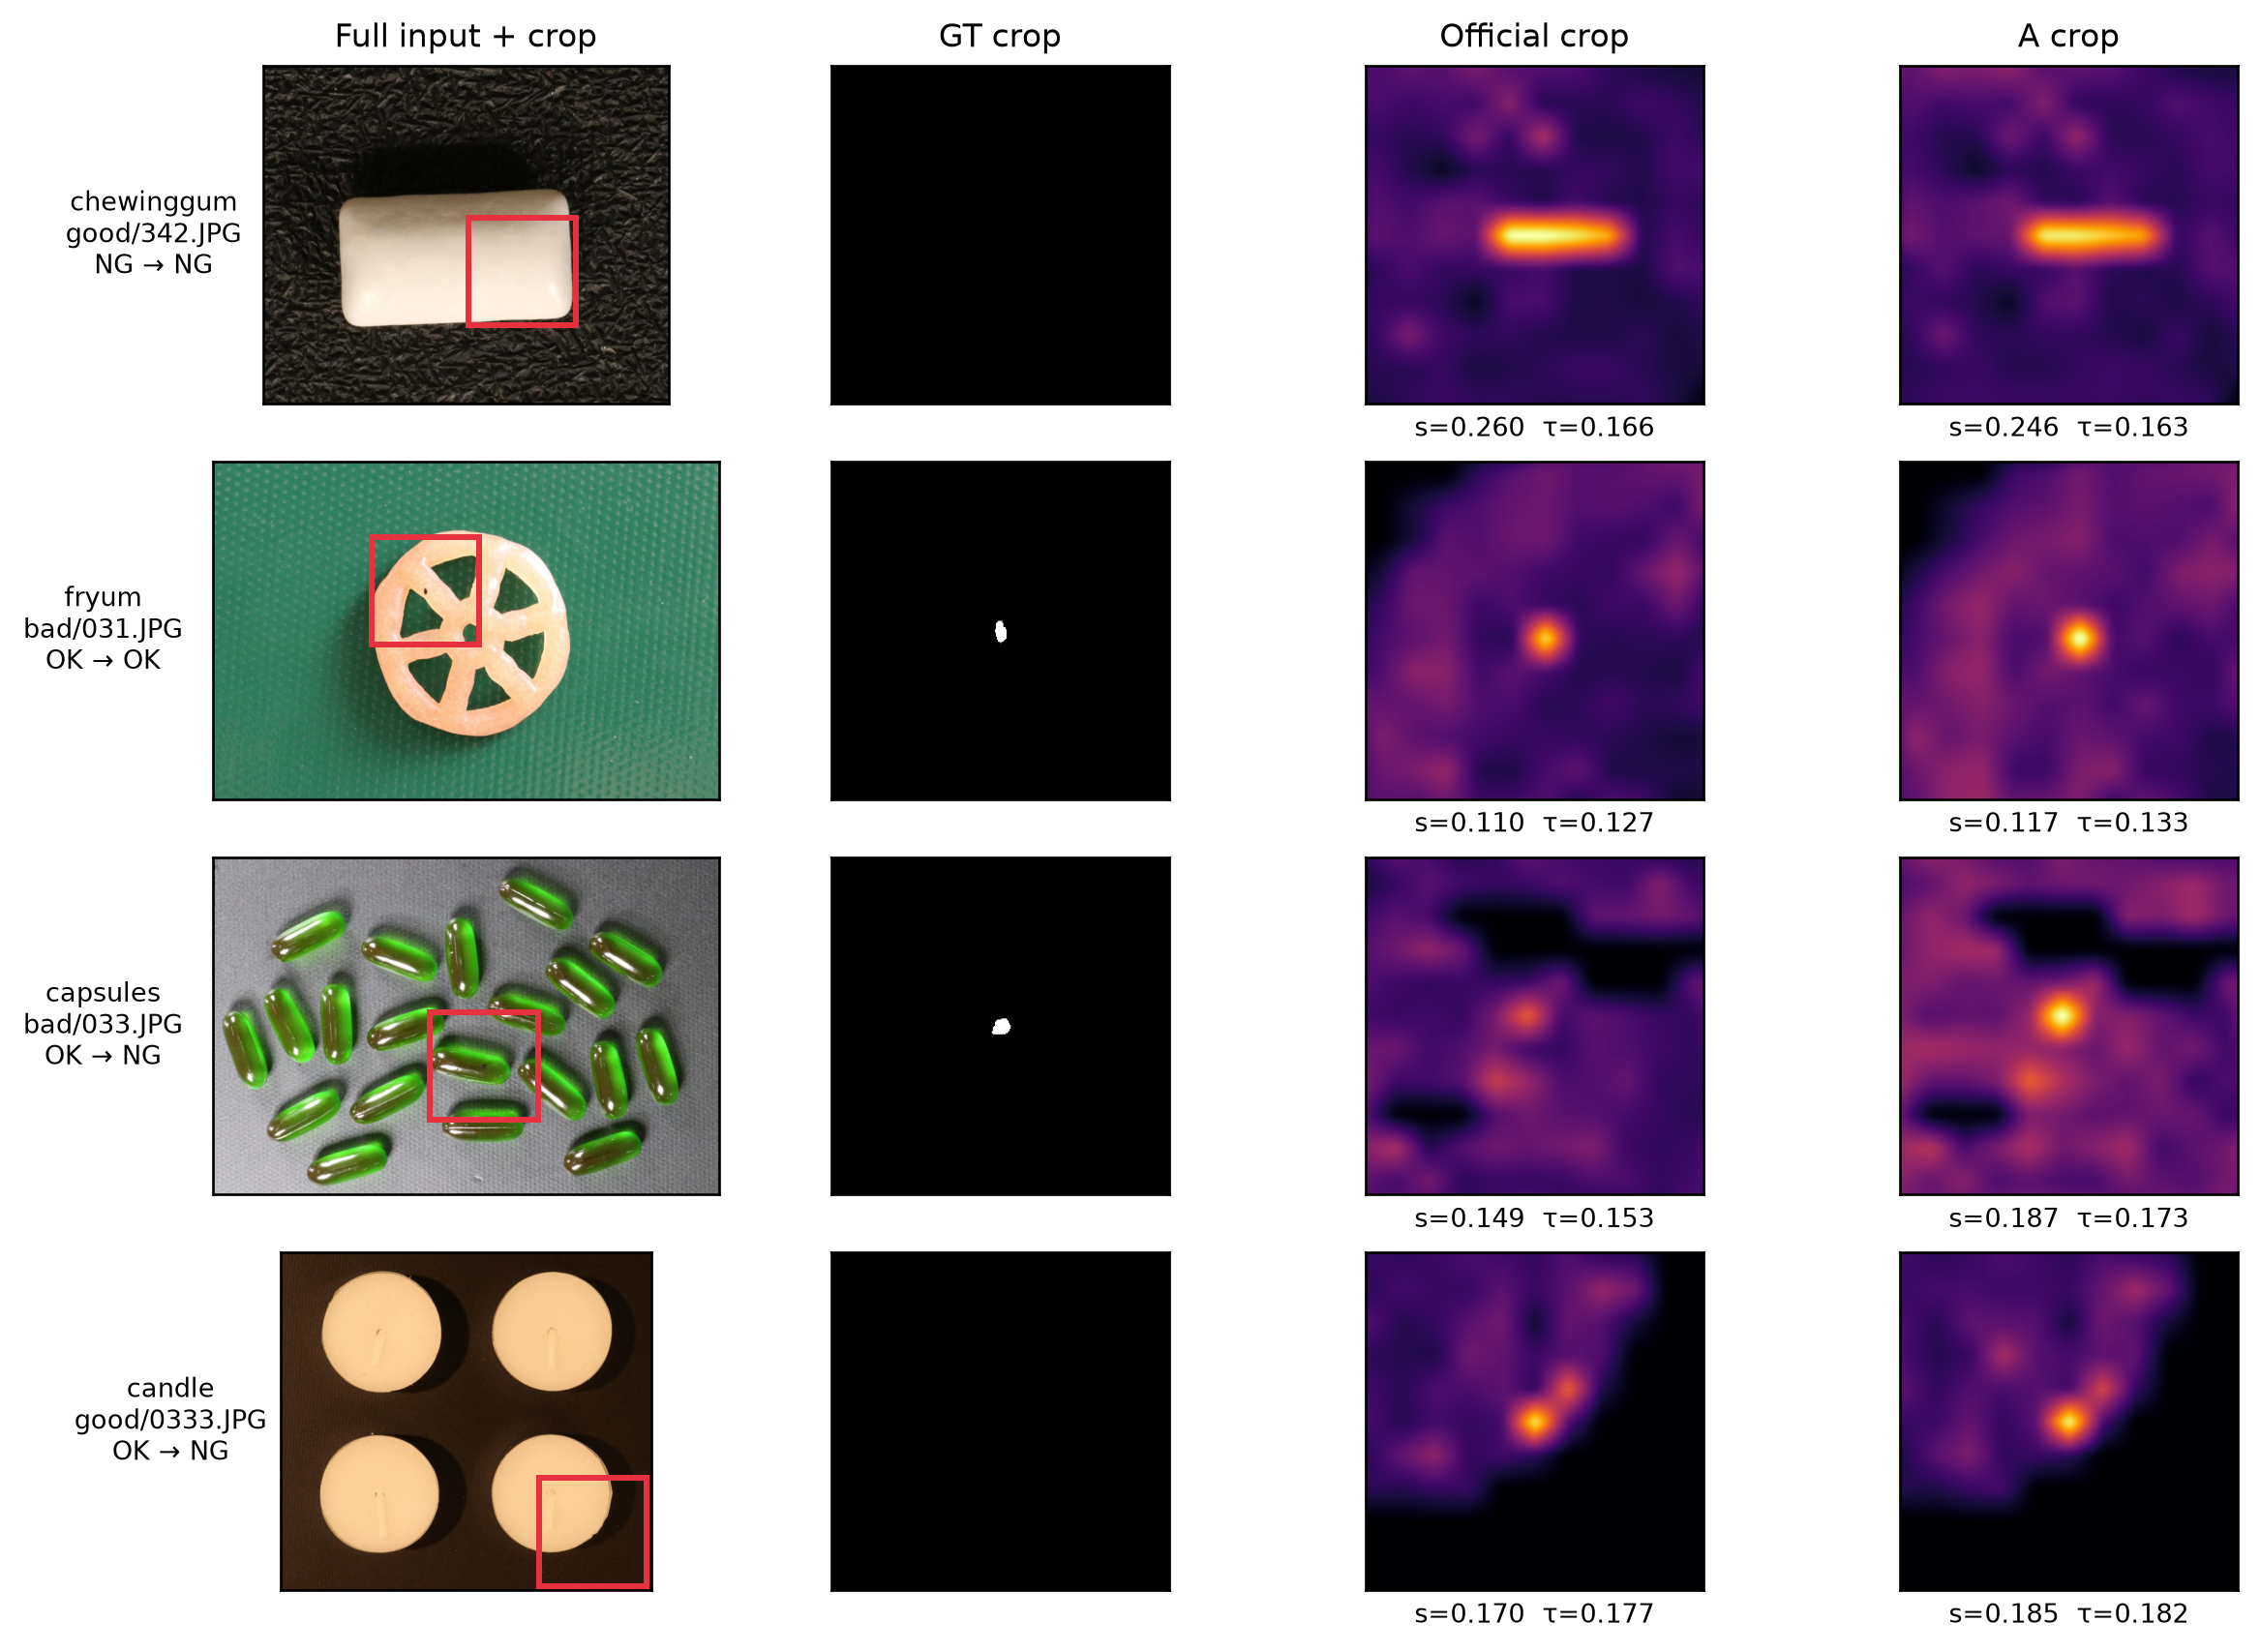
\includegraphics[width=.98\textwidth]{figures/difficult_cases_2.png}
  \caption{A normal chewinggum false positive, a small fryum false negative, a corrected capsules defect, and a newly false-alarmed normal candle (\texttt{TN}\,$\rightarrow$\,\texttt{FP}). Each score is paired with its own normal-calibrated threshold $\tau$. Black masks for normal cases are expected. Crops are for presentation only; decisions use full images.}
  \label{fig:cases2}
\end{figure*}

Two-layer A increases image AUROC at every shot count, but the gain is modest: $+0.13$, $+0.14$, $+0.30$, and $+0.23$ percentage points. At four shots the paired group-level gains are $+0.46$, $+0.28$, and $+0.17$ points, so there is no claim of a large or uniform effect. At one shot the pixel mean declines by 0.05 points; at two shots it is almost unchanged. The later pixel gains are only 0.03 and 0.04 points, computed from the displayed two-decimal means. Earlier features can change image-level ordering without reliably solving fine segmentation.

\subsection{Per-category behavior and decisions}
Table~\ref{tab:category} exposes variation hidden by the macro mean. At four shots, image AUROC improves in all six categories, but pixel AUROC falls for capsules and cashew. The larger pipe\_fryum image gain does not prove every defect type improves. For thresholded decisions, the same four-shot/group-0 six-category set contains 19 official false negatives converted to true positives by A, while some formerly correct cases regress. We report both directions in the per-image CSV rather than optimizing a threshold on test labels. Image AUROC evaluates ranking; a normal-calibrated threshold can still miss a visible response.

Aggregating all three four-shot reference groups gives the transition counts in Table~\ref{tab:transitions}. These are 2,880 \emph{predictions} of 960 unique images, not 2,880 independent test images. A corrects 62 original mistakes (39 missed defects and 23 false alarms) but creates 78 new mistakes (27 missed defects and 51 false alarms). Of the 51 new false alarms, candle contributes 18, capsules and chewinggum 10 each, pipe\_fryum 8, fryum 4, and cashew 1. The 27 new missed defects split as candle 9, cashew and fryum 7 each, capsules 2, and chewinggum and pipe\_fryum 1 each. Thus its AUROC gain does not translate into better accuracy at our fixed normal-only threshold. Calibration on 20 normals may not characterize all legitimate product variation.

\begin{table}[t]
\centering
\caption{Four-shot thresholded decision transitions from official DINO to A, pooled over three reference groups. The deployed threshold uses normal calibration only; ground truth determines these retrospective labels.}
\label{tab:transitions}
\small
\begin{tabular}{l r l r}
\toprule
Correction & Count & Regression & Count\\
\midrule
FN $\rightarrow$ TP & 39 & TP $\rightarrow$ FN & 27\\
FP $\rightarrow$ TN & 23 & TN $\rightarrow$ FP & 51\\
\bottomrule
\end{tabular}
\end{table}

\begin{table*}[t]
\centering
\caption{Four-shot AUROC (\%) by category, averaged over three matched groups. $\Delta$ is A minus Official in percentage points from the displayed means; black underlining marks the better paired score.}
\label{tab:category}
\small
\setlength{\tabcolsep}{3.7pt}
\begin{tabular}{l r rrr rrr}
\toprule
Category & Template image & DINO image & A image & $\Delta$ image & DINO pixel & A pixel & $\Delta$ pixel\\
\midrule
candle & 59.00 & 92.80 & \bestscore{92.90} & +0.10 & 98.36 & \bestscore{98.45} & +0.09\\
capsules & 60.72 & 98.06 & \bestscore{98.38} & +0.32 & \bestscore{95.37} & 94.93 & $-0.44$\\
cashew & 57.28 & 93.31 & \bestscore{93.61} & +0.30 & \bestscore{99.23} & 99.17 & $-0.06$\\
chewinggum & 51.53 & 98.95 & \bestscore{99.05} & +0.10 & 99.55 & \bestscore{99.59} & +0.04\\
fryum & 66.83 & 97.41 & \bestscore{97.77} & +0.36 & 96.93 & \bestscore{97.31} & +0.38\\
pipe\_fryum & 51.44 & 96.38 & \bestscore{97.01} & +0.63 & 99.12 & \bestscore{99.25} & +0.13\\
\midrule
Macro & 57.80 & 96.15 & \bestscore{96.45} & +0.30 & 98.09 & \bestscore{98.12} & +0.03\\
\bottomrule
\end{tabular}
\end{table*}

\begin{table}[t]
\centering
\caption{Exact original-resolution four-shot pixel AP (\%) across three fixed reference groups. The final row is sample SD of category-macro scores; black underlining marks the best macro mean. Normal test masks are zero; AnyUp changes maps, not image scores.}
\label{tab:pixelap}
\small
\begin{tabular}{lrrr}
\toprule
Category & Official & A & A+AnyUp\\
\midrule
candle & 31.03 & 31.04 & 38.77\\
capsules & 40.73 & 40.02 & 54.83\\
cashew & 57.71 & 56.11 & 67.59\\
chewinggum & 71.95 & 71.39 & 77.39\\
fryum & 40.99 & 43.78 & 54.14\\
pipe\_fryum & 45.17 & 49.22 & 59.44\\
\midrule
Macro mean & 47.93 & 48.59 & \bestscore{58.69}\\
Macro sample SD & 0.48 & 0.30 & 0.38\\
\bottomrule
\end{tabular}
\end{table}

Pixel AUROC near 98\% masks variation in precision on sparse defect pixels. Across three four-shot reference groups, A changes macro pixel AP only from 47.93$\pm$0.48\% to 48.59$\pm$0.30\%; capsules and chewinggum regress. Applying pretrained AnyUp to A's maps raises AP to 58.69$\pm$0.38\% (Table~\ref{tab:pixelap}). This is a repeated-reference localization gain, not a better image decision: AnyUp acts after retrieval and leaves each image score and threshold unchanged.

In a post-hoc four-shot/group-0 layer diagnostic, block 11 alone scores 95.84\% image AUROC and block 8 alone 95.88\%; equal block 8+11 scores 96.29\%. Equal block 5+11 is nearly tied at 96.28\%, while 10+11 is 96.10\%. Block 8 weights of 0.25 and 0.75 score 96.09\% and 96.28\%. This single-group test diagnostic supports possible layer complementarity, not a claim that block 8 or equal weighting is optimal. It did not select pre-fixed A.

\subsection{Efficiency and localization ablation}
Table~\ref{tab:efficiency} measures all five paths in one paired query run. A adds 86.68 ms/image (31.5\%) over official DINO, with similar peak allocated GPU tensor memory. Both descriptors come from one frozen backbone pass; the 384-to-768-dimensional bank plausibly makes CPU nearest-neighbor search the dominant added cost. The independently synchronized stage diagnostic below tests this explanation. The separate pretrained AnyUp experiment redistributes \emph{existing} patch anomaly scores by $2\times$ before unchanged original-resolution restoration~\cite{wimmer2026anyup}. It leaves image scores and decisions exactly unchanged. Across three four-shot groups, official+AnyUp pixel AUROC is 98.64\%, versus 98.09\% for direct restoration and 98.29\% for a matched two-step bilinear control. A+AnyUp reaches 98.63$\pm$0.05\% pixel AUROC across the same three groups; the timing table covers group 0 only.

The separate CPU RGB template baseline averages 28.21 ms/image (0 MiB GPU); its timing boundary differs from Table~\ref{tab:efficiency}.

\begin{table}[t]
\centering
\caption{One synchronized, warmed 120-query run, four shots/group 0, RTX 4060 Laptop GPU. All five paths include decode, extraction, retrieval, and restoration; setup and output are excluded. Peak allocated GPU tensor memory includes resident weights.}
\label{tab:efficiency}
\small
\begin{tabular}{lrr}
\toprule
Query path & ms/image & Peak MiB\\
\midrule
Official DINO 448 & 274.92 & 208.28\\
Two-layer A 448 & 361.59 & 210.53\\
A + AnyUp & 528.93 & 1074.06\\
Official DINO 672 & 679.71 & 244.33\\
Fixed 448+672 & 950.95 & 244.33\\
\bottomrule
\end{tabular}
\end{table}

An independently synchronized stage diagnostic on the same 120 query files measures 86.2$\rightarrow$160.6 ms for CPU FAISS search, 68.3$\rightarrow$74.9 ms for feature extraction, 9.5$\rightarrow$9.8 ms for masking/normalization, and 71.6$\rightarrow$68.8 ms for scoring/map restoration (official$\rightarrow$A). Decode/preprocessing is 41.6$\rightarrow$42.5 ms. Most added time in that diagnostic is retrieval, consistent with doubled vector width. Its stage sums (277.2/356.6 ms) are close to, but methodologically distinct from, the unified query times; the two protocols must not be mixed. Direction E's 25\% bank is one possible speed trade-off, but its weaker image AUROC does not solve the problem.

\subsection{Qualitative errors and corrected case}
We distinguish (i) small defects diluted within a patch (cashew \texttt{bad/063} and fryum \texttt{bad/031}); (ii) visible local response whose top-1\% image score stays below $\tau$ (candle \texttt{bad/000} and capsules \texttt{bad/087}); (iii) normal appearances outside a small reference bank (chewinggum \texttt{good/342}); and (iv) an intermediate-layer-induced normal false alarm (candle \texttt{good/0333}). These are diagnostic interpretations of displayed cases, not causal isolation experiments.

Figures~\ref{fig:cases1} and~\ref{fig:cases2} show seven fixed four-shot/group-0 cases. Each row uses one shared heatmap scale for official and A. Red boxes mark display crops; masks guide crops \emph{only for illustration}. Candle \texttt{bad/000.JPG}, capsules \texttt{bad/087.JPG}, cashew \texttt{bad/063.JPG}, and fryum \texttt{bad/031.JPG} remain false negatives under both normal-calibrated decision rules. The heatmaps can respond near a defect but still yield image scores below threshold; neither response nor its visualization alone proves a correct detection. Chewinggum \texttt{good/342.JPG} remains a false positive, illustrating that a normal local appearance may be distant from a small reference bank. Conversely, capsules \texttt{bad/033.JPG} changes from a false negative to a true positive under A; while new false alarms show that the gain does not generalize uniformly.

A post-hoc aggregation check recalibrates the 95th-percentile normal threshold for each top-$k$ patch fraction on the same three four-shot groups. Narrowing official DINO's top 1\% to 0.5\% raises image AUROC from 96.15$\pm$0.49\% to 96.46$\pm$0.64\%, but errors rise from 365 to 368 over 2,880 decisions. At 0.1\%, errors rise to 376. Candle \texttt{bad/000} and capsules \texttt{bad/087} remain missed in group 0 under all fractions tested. Thus the displayed response does not establish that top-1\% dilution alone causes these failures; the diagnostic is test-informed and not a validated replacement score.



\FloatBarrier
\section{Additional Directions and Limitations}
\label{sec:additional}
A remains the pre-fixed primary comparison. Secondary methods differ in supervision and scope: four-shot equal-score DINO+AnomalyCLIP fusion reaches 96.57\% image AUROC versus A's 96.45\%, winning only 9 of 18 category/group pairs. AnomalyCLIP uses external MVTec AD anomaly labels and no VisA reference sampling; its standalone image/pixel AUROC is 89.54/95.81\%. The later review gate is exploratory, not an equal-supervision few-shot accuracy gain.

\subsection{Image scale and defect strata}
Tiny-defect misses motivated a post-hoc second image scale. We ran frozen DINOv2 at a 672-pixel short edge and equally averaged its threshold-normalized score with the original 448 branch. Both use identical reference filenames; the fused threshold uses the same 20 paired normal calibration images. No test label sets weights or thresholds. Table~\ref{tab:multiscale} covers all shots/groups, but the candidate arose after inspecting this test split and lacks independent validation.

\begin{table}[t]
\centering
\caption{Six-category macro image AUROC (\%, mean$\pm$sample SD over groups 0--2). The lower panel compares the post-hoc 672 branches on the same test split; black underlining marks the larger row mean.}
\label{tab:multiscale}
\scriptsize
\setlength{\tabcolsep}{3pt}
\begin{tabular}{lrr}
\toprule
Shots & Official & A\\
\midrule
1 & 94.61$\pm$1.03 & 94.74$\pm$0.99\\
2 & 95.33$\pm$0.57 & 95.47$\pm$0.54\\
4 & 96.15$\pm$0.49 & 96.45$\pm$0.38\\
8 & 96.62$\pm$0.70 & 96.85$\pm$0.74\\
\bottomrule
\end{tabular}\par\vspace{3pt}
\begin{tabular}{lrr}
\toprule
Shots & 672 & 448+672\\
\midrule
1 & 94.97$\pm$0.38 & \bestscore{95.49$\pm$0.54}\\
2 & 95.76$\pm$0.38 & \bestscore{96.12$\pm$0.39}\\
4 & 96.29$\pm$0.24 & \bestscore{96.74$\pm$0.27}\\
8 & 96.82$\pm$0.56 & \bestscore{97.22$\pm$0.60}\\
\bottomrule
\end{tabular}
\end{table}

\begin{table}[t]
\centering
\caption{Four-shot official $\rightarrow$ 448+672 decision changes over three groups. Columns are corrected/missed defects and corrected/new false alarms, respectively; all four directions are reported.}
\label{tab:scale_transitions}
\scriptsize
\setlength{\tabcolsep}{3pt}
\begin{tabular}{lrrrr}
\toprule
Class & FN$\to$TP & TP$\to$FN & FP$\to$TN & TN$\to$FP\\
\midrule
candle & 7 & 1 & 5 & 27\\
capsules & 16 & 0 & 2 & 4\\
cashew & 20 & 4 & 0 & 0\\
chewinggum & 0 & 4 & 4 & 8\\
fryum & 5 & 2 & 4 & 5\\
pipe\_fryum & 1 & 1 & 4 & 9\\
\midrule
Total & 49 & 12 & 19 & 53\\
\bottomrule
\end{tabular}
\end{table}

\begin{table}[t]
\centering
\caption{Four-shot defect-area audit over three groups. Image AUROC and recall compare each anomalous stratum against all category normals; pixel AP includes those normals. Large defects occur in four classes only. AP prevalence differs across strata.}
\label{tab:size_strata}
\scriptsize
\setlength{\tabcolsep}{3pt}
\begin{tabular}{llrrr}
\toprule
Area & Method & Im. AUROC & Recall & Pixel AP\\
\midrule
\multirow{3}{*}{$<0.5\%$} & 448 & 95.18 & 85.66 & 30.08\\
 & A & 95.64 & 86.64 & 31.21\\
 & 448+672 & 95.96 & 88.17 & 35.43\\
\multirow{3}{*}{$0.5$--$2\%$} & 448 & 99.87 & 99.25 & 58.92\\
 & A & 99.77 & 99.40 & 59.04\\
 & 448+672 & 99.80 & 99.40 & 62.68\\
\multirow{3}{*}{$>2\%$} & 448 & 100.00 & 100.00 & 75.68\\
 & A & 100.00 & 100.00 & 78.09\\
 & 448+672 & 100.00 & 100.00 & 78.92\\
\bottomrule
\end{tabular}
\end{table}

At four shots, fixed fusion raises image AUROC from 96.15$\pm$0.49\% to 96.74$\pm$0.27\% and exact pixel AP from 47.93$\pm$0.48\% to 51.89$\pm$0.65\%. Its pixel AUROC over 1/2/4/8 shots is 98.19/98.32/98.46/98.56\%, versus official 97.76/97.92/98.09/98.21\%. Of 600 distinct anomalies, 439 occupy under 0.5\% of the image. Table~\ref{tab:size_strata} reports all defect-area bins; AP prevalence differs by bin. At four shots, the fusion corrects 49 missed defects but loses 12 previously detected defects; it also clears 19 false alarms while creating 53 (Table~\ref{tab:scale_transitions}). Thus thresholded errors fall only from 365 to 362 across 2,880 repeated-group decisions. Chewinggum and pipe\_fryum regress, so the ranking gain is neither universal nor a large decision gain. Pretrained A+AnyUp has stronger four-shot pixel AP (58.69$\pm$0.38\%) but cannot alter image decisions.

\subsection{Calibration and selective review}
A 200-resample normal-only bootstrap compared empirical 95th-percentile, Gaussian, and fitted Gumbel thresholds across 18 four-shot category/group settings, each with 20 disjoint normal calibration scores. For 448, their mean bootstrap threshold SDs are 0.0154/0.0099/0.0094, with retrospective test FP/FN totals 154/211, 152/194, and 142/190. For 448+672, the corresponding SDs are 0.0796/0.0523/0.0512 and FP/FN totals 188/174, 186/178, and 183/180. Score units differ across the two methods; 20 samples cannot establish Gaussian or Gumbel assumptions, and test errors cannot select a deployed estimator. A DINO-only review audit sends 10\% of images closest to the normal-calibrated boundary to a human; automatic-decision error is 10.39\% for 448 and 9.25\% for 448+672. Reviewed cases remain unresolved.

\subsection{Exploratory directions and limitations}
Direction F instead reviews externally supervised DINO+AnomalyCLIP scores. Its fixed band queues 426/2,880 four-shot decisions (14.79\%), including 80/180 missed defects. These are \emph{reviewed misses}, not true positives. At retrospective 90\% coverage, automatic-decision error is 8.84\% versus original DINO's 10.39\%; the margin is not a calibrated correctness probability.

B/C/E use only four shots/group 0 and score 95.50/83.69/95.64\% image AUROC, versus 95.84\% for matched official DINO. B retains 38\% of bank patches; C uses four real normal and 32 synthetic images per class; E's 25\% bank shortens isolated FAISS search from 103.54 to 26.55 ms. None establishes a three-group or pixel-level gain, and E's retrieval speedup is not end-to-end.

The optional autoencoder trains on 2,813 normals with 312 validation images across three training seeds, outside the few-shot protocol; image/pixel AUROC is 82.74/69.59\%. Reconstruction does not ensure precise boundaries. Repeating deterministic AnomalyCLIP inference is not a three-reference-group stability test. Both use 20 normal demo-calibration images.

Limitations include coarse patches, remaining threshold errors, added runtime, and no independent holdout for exploratory selection. AnyUp improves localization but increases time and memory. Six classes do not establish factory-wide generalization. Saved filenames, calibration scores, maps, and per-image decisions support audit.

\FloatBarrier
\section{Conclusion}
\label{sec:conclusion}
Frozen AnomalyDINO greatly exceeds the RGB template baseline. Pre-fixed A gives a small image-AUROC gain with little pixel-AP change and higher retrieval cost. Post-hoc scale fusion improves ranking and tiny-defect recall but costs 3.46$\times$ query time and reduces four-shot errors by only three across repeated groups. AnyUp improves localization without changing image decisions. Next, an untouched validation split should guide variant selection, efficient fine-scale matching, and normal-only calibration under a fixed review budget. \href{https://github.com/yedaojun/AIAA3201-Project-2}{Code and results} are available.

{\small
\bibliographystyle{ieeenat_fullname}
\bibliography{references}
}

\end{document}
